\subsection{Le besoin de la communauté}

Pour que le projet soit un succès, il est nécessaire de répondre à certains besoins de la future communauté. Le psychologue Abraham Maslow a développé en 1940 une théorie concernant la motivation des individus et il affirme que chaque action est motivée selon un besoin bien particulier.
Dans sa théorie, Maslow répartit les différents besoins en cinq catégories :
\begin{itemize}
	\item besoin physiologique (faim, soif, respiration, reproduction...)
	\item besoin de sécurité (recherche d'un environnement stable)
	\item besoin d'appartenance et d'amour
	\item besoin d'estime (confiance en soi, reconnaissance et appréciation)
	\item besoin d'accomplissement
\end{itemize}

Ces besoins sont répartis selon le diagramme suivant, en couche successive par ordre d'importance. Pour que l'impact soit fort, il est nécessaire de toucher le futur candidat sur une ou plusieurs de ces catégories afin de susciter chez lui une envie de rejoindre le département ASI de l'INSA de Rouen.

\begin{center}
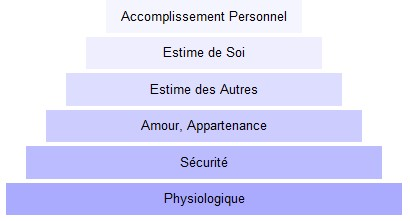
\includegraphics[scale=0.5]{./image/pyramidemaslow.jpg}
\end{center}
~~\\
\indent Le but de notre projet est de donnée une meilleure visibilité au département ASI afin de donner envie aux potentiels candidats de postuler. Clairement, les deux premières catégories ne font pas partie des besoins que la présence du département ASI sur les réseaux sociaux peut satisfaire (même si la formation permet de "mettre du beurre dans les épinards"). ~~\\
\indent En revanche les trois dernières sont beaucoup plus à portée. 
\indent De part l'ambiance "école" de l'INSA de Rouen, et des diverses rencontres du groupe INSA plus généralement, le futur postulant va souhaiter intégrer le département et ainsi faire partie du groupe. ~~\\
\indent Le département ASI, même si moins bien coté que le département IF de l'INSA de Lyon reste une formation d'excellence et prestigieuse. Cette reconnaissance est tout à fait à même de satisfaire le besoin d'estime du futur postulant. ~~\\
\indent Enfin, le besoin d'accomplissement est certainement l'axe majeur de la formation d'ingénieur ASI dans la mesure où celui-ci sera amené, lors de la formation, comme durant toute sa carrière professionnelle de développer et mettre en place des projets de grande envergure.

\subsection{Rayonner sur le web et fidéliser un utilisateur}
\subsubsection{Capitaliser sa communauté}
Pour réussir à rayonner sur internet, il est nécessaire de créer une communauté et de la fidéliser. Pour créer une communauté, une solution pourrait être d'envoyer à un spectre très large de personnes un lien vers notre page. Sur ces personnes, beaucoup ne liraient pas le message, peu iraient sur la page, et encore moins le partageraient. Il faut donc trouver quelques éléments, dès le départ, actifs, qui seraient vecteur de propagation d'informations auprès de leurs contacts. Cette communauté serait alors amené à grossir de façon saine et pérenne par bouche à oreille.
\paragraph{}
De plus, ajouter des boutons de partages sur le site web asi.insa-rouen.fr, ainsi que sur toutes les actualités diffusés permet aux lecteurs de partager eux même l'information, et ainsi de s'impliquer dans l'impact que peut avoir la présence du département ASI sur les réseaux sociaux. Ces boutons permettrons aussi aux visiteurs du site de s'abonner aux publications sans passer par le moteur de recherche des réseaux sociaux et ainsi gagner en temps. Facile et rapide, cette fonction apporte toujours un plus et touchera un publique plus large en donnant l'information aux possibles intéressés, comme aux simples visiteurs, que le département est présent sur les réseaux sociaux.
\subsubsection{Twitter}
Le nombre de 'followers' n'est pas une fin en soit. Il est possible de gonfler ces statistiques en achetant de faux comptes et des grossistes vendent des followers par pack de 50 000. Un compte Twitter efficace et efficient est un compte dont les tweets sont retweeté et commenté. Et pour être vu sur Twitter, il faut être retwitté, partagé.
\paragraph{}
Le graphique ci-dessous montre la chance d'un tweet d'être partagé en fonction de son contenu. Il apparait que les tweets contenant des liens vers des photos ou des vidéos, sont deux fois plus partagés que les tweets ne contenant que du texte.
\begin{center}
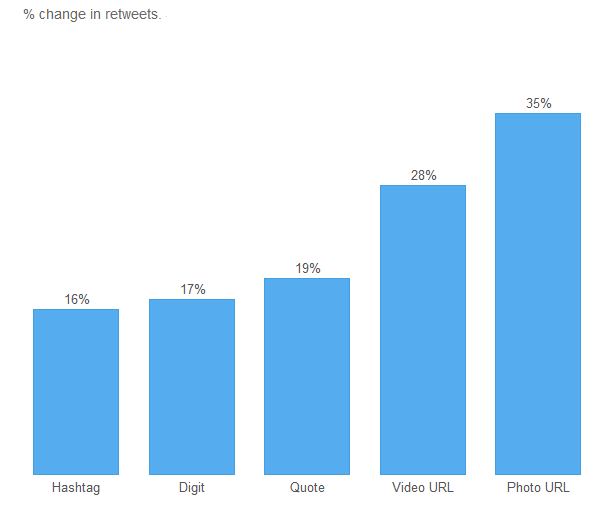
\includegraphics[scale=0.5]{./image/retweet.png}
\end{center}

\paragraph{Tweeter par Twitter ~~\\} 
Dans son guide, Twitter recommande de tweeter régulièrement afin de garder une page active et suggère de suivre la base d'un tweet quotidien.
Il existe de nombreux sujets qu'il est possible de relayer via Twitter.
\begin{itemize}
	\item informations insolites (robots puissance4)
	\item astuces utiles (offre de tel ou tel compagnie pour les étudiants)
	\item information de fonctionnement (rentrée, choix des PICs)
	\item retweet d'information sur le département ou l'insa (article de journal)
	\item mise en avant de personnalité (gagnant de concourt, personnel du département)
	\item information sur l'actualité relative au domaine ASI
\end{itemize}
\paragraph{}
 Les gens partagent plus facilement les tweets qui les amuses, qui répondent à leurs questions ou les inspirent. Le twitter du département doit se placer comme un relai d'information et comme maitre à penser dans son domaine. Pour s'offrir une telle visibilité, il sera nécessaire de suivre les incontournables du secteur (groupe et personnalité) et d'établir des liens avec eux.
\subsubsection{Facebook}
Créer une fanpage sur Facebook permet une visibilité permanente, car dès qu'une information est publiée, elle apparait sur le mur de chaque fan. C'est certainement l'un des moyens les plus efficaces et les plus puissant de fidéliser à l'heure actuelle. Cependant, l'algorithme edgerank utilisé par facebook, ne permet pas aux posts d'être partagé à l'infinie. Seuls les posts possédant un grand nombre de mentions "j'aime", de partage et de commentaire sont partagé à l'ensemble des fans. Afin que les informations soient relayées au plus grand nombre, la communauté doit être actives afin de faire sortir le contenu de la page pour le diffuser largement.
\paragraph{}
Sur facebook, les contenus provoquant le plus d'engagement (likes, partages ou commentaires) sont les partages d'image et de vidéo. Cependant, les status ont la portée la plus grande et seront plus susceptible de passer la barrière de l'edgerank. Ainsi, il est nécessaire de créer du contenu sans média pour avoir un impact et attirer les fans 'inactifs' a commenter la page, et en simultané, de publier photos et vidéos afin de suscité l'intérêt de la communauté qui partagera se contenu par la suite.